\documentclass[11pt, a4paper]{article}

\usepackage{url}
\usepackage{cite}
\usepackage{times}
\usepackage{float}
\usepackage{caption}
\usepackage{courier}
\usepackage{hyperref}
\usepackage{breakurl}
\usepackage{graphicx}
\usepackage{fancyhdr}
\usepackage{boolexpr}
\usepackage{multirow}
\usepackage{subfigure}
\usepackage{indentfirst}
\usepackage[inline]{enumitem}

% no color links
\hypersetup{
bookmarks=false,
colorlinks=true,
citecolor=black,
filecolor=black,
linkcolor=black,
urlcolor=black,
pagebackref=true
} 

% compact bibliography
\let\oldthebibliography=\thebibliography
\let\endoldthebibliography=\endthebibliography
\renewenvironment{thebibliography}[1]{	%
	\begin{oldthebibliography}{#1}	%
	\setlength{\parskip}{0ex}	%
	\setlength{\itemsep}{0.4ex}	%
  \fontsize{7.1}{8.5}
  % tweak label width for proper alignment - two digits
  \settowidth\labelwidth{\@biblabel{99}}
	\selectfont
}{\end{oldthebibliography}}

% hacks
\newcommand{\note}[1]{\noindent\textbf{\color{red}[#1]}}
\newcommand{\comment}[1]{}

\title{\Large \bf \underline{Challenge:}\\
How might we have more transparency on where our data is going in the Internet?\\}
\author{
	Petros Gkigkis\\
	\texttt{gkigkis@ics.forth.gr}\\
	\and
  	Konstantinos Kleftogiorgos\\
	\texttt{kleftog@ics.forth.gr}\\
	\and
	Natasa Ntagianta\\
	\texttt{dagianta@csd.uoc.gr}\\
  	\and
	Eva Papadogiannaki\\
  	\texttt{epapado@ics.forth.gr}\\
	\and
	Nestoras Sdoukos\\
	\texttt{sdoukos@csd.uoc.gr}\\
	\and
	Kostas Solomos\\
	\texttt{solomos@ics.forth.gr}\\
	\and
	Antonis Tzougkarakis\\
	\texttt{tzugarak@csd.uoc.gr}\\
}
\date{}

\pagestyle{fancy}
\fancyhf{}
\rhead{}
\lhead{CS-533: Security, Privacy and Intelligence on the Internet}
\rfoot{Page \thepage}

\begin{document}

	\pagenumbering{gobble}
	\maketitle
	\newpage
	\pagenumbering{arabic}

	\section{Chapter 2: Ideation}
	\subsection{Synthesis}
	\subsection{Questionnaire findings}

The first finding was that, the majority  of the respondents feel at most 
moderately safe on the Internet as 41.5\% of them chose the typical answer. 
Another result from the questionnaire was that internet users believe that the 
protection of their information is not very strict with a percentage of 43.1\%. 
However, even if users believe that there isn't any stringency to the user 
information on the Internet, one in two users do care about their privacy. 
One third of the users have basic knowledge on data transparency and a 
percentage of 47.7\% is aware that their personal information might be leaked on 
the internet even though they are not hacked. 

Concerning whether users care where the companies store their data, the answers 
were divergent. Furthermore, users  tend to care how their traffic is routed 
through the Internet being indicated by the fact that half of them gave a 
corresponding answer. In addition, users care a lot about the identity of the 
third party companies and ISPs through which their traffic is routed. 
A very high percentage of the respondents are being aware that their data can 
traverse through multiple countries. 

Although, they know that their data are traversing multiple countries they are 
not fully aware that legislations of these countries may apply on them, as the 
findings are divergent. A small percentage of the users, specifically 4,6\%, are 
highly informed about the impact of the internet laws on their data. 
On the other hand, approximately 50\% of users care a lot about  the information 
shared by their ISP's to law enforcement agencies and government. Moreover, 
another finding states that very few of the users pay attention to the terms and 
agreements of the Internet Service Providers and online services.

More than 50\% of the responders are fully aware of the existence of targeted 
ads on the Internet, and the role of profiling and tracking entities. On the 
other hand, the answers on how aware of the way the targeted ads work are 
varying and towards high. Their treatment as products tend to concern users a 
lot at a percentage of 40\%. 

A diversity of the users trusting the Internet Service Providers tends to be 
pretty low. This leads users to not trusting the privacy of their information on 
social media at a percentage of 50\%. Regarding the anonymization tools users 
tend to be aware that they exist. In addition, the 20\% are fully aware of their 
existence. Finally, concerning whether the users are willing to pay for 
anonymization tools and privacy services, the answers are contradictory, but 
display a positive attitude towards it.

\subsection{Interview findings}

The first finding of the interview is that despite the existing laws, there is 
not a single authority in charge of enforcing them. It is established by the law 
that a warrant is mandatory, for someone to acquire access to  user's data. 
However, there is not a responsible authority to impose penalties in case of any 
illegality.

In addition, we found out that ISPs indeed scan and utilize the incoming and 
outcoming traffic with various mechanisms. Those mechanisms include but are not 
limited to splitters, tapping, NetFlow and SFlow.

Regarding data storage mechanisms, ISPs store data in order to ensure the user's 
security, by detecting and preventing malicious activities. The data are not 
used for advertising reasons.

Moreover, regarding the surveillance there is little information about the exact 
location of the tapping. Surveillance locations, there are not enough 
information revealing their locations, although some insight can be inferred 
from leaked documents. There are submarines and robots, built by the army, that 
act as surveillance mechanisms and are more difficult to be discovered and 
prevented.  There are many researchers working on how to discover the peering 
matrices inside IXPs. Furthermore, there are databases providing this kind of 
information but they might be inaccurate due to the continually change of IXP 
member list.


	%\input{ch2_sec2}
	\subsection{Key insights} 

\vspace{0.4cm}
\paragraph{Theme:} Privacy and anonymization tools.
\paragraph{Insights:}
\begin{enumerate}
\item
Users regardless of age or education level tend to care about their privacy on 
the internet.
\item
The majority of users believe that there isn't any stringency on user's internet 
data privacy.
\item
Even though users are willing to use anonymization tools for their protection on 
the internet, they seem reluctant to pay for such a service.
\end{enumerate}

%%
\vspace{0.1cm}
\paragraph{Theme:} Routing and Storage. 
\paragraph{Insights:}
\begin{enumerate}
\item
Most of the users seem to be concerned about their traffic routing and data and 
the specific storage locations.
\item
Users want to be more informed about the identity of third party companies 
interceding their communications.
\end{enumerate}

%%
\vspace{0.1cm}
\paragraph{Theme:} Law Enforcements and Regulations.
\paragraph{Insights:}
\begin{enumerate}
\item
Users tend to not pay attention to the ISPs terms and agreements regardless of 
the time they have spent on the internet. 
\item
More than half of users, care a lot about the sharing of their information to 
the law enforcement agencies and government.
\item
Users are not fully informed about the implication of laws of each country on 
their data.
\end{enumerate}

%%
\vspace{0.1cm}
\paragraph{Theme:} Economy and Advertising. 
\paragraph{Insights:}
\begin{enumerate}
\item
Users are fully aware of the existence of targeted advertising on the internet.
\item
Users are aware about profiling mechanisms on targeted advertising, and they are 
concerned about being the product of the internet advertising companies. 
\end{enumerate}

%%
\vspace{0.1cm}
\paragraph{Theme:} User Trust. 
\paragraph{Insights:}
\begin{enumerate}
\item
Most of the users tend to not trust the ISPs with handling their personal 
information.
\item
A very high percentage of the users do not trust the social media to keep their 
information private.
\end{enumerate}


	\subsection{Refining challenges}
\label{section_4}

\paragraph{Insight: } 
Users tend to not pay attention to the ISPs terms and agreements regardless of 
the time they have spent on the internet. \\
\\\emph{How might we } 
refine terms and agreements more appealing to users and engage them more to pay 
attention to what they have agreed with?

\paragraph{Insight: }
Users are concerned about their profiling on targeting advertisement. \\
\\\emph{How might we }
restrict profiling to provide targeted advertising only on the services that 
will benefit us, regarding user budget and targeted recommendations (e.g. 
e-shops, airline tickets)?\\
\\\emph{How might we }
have more transparency on the exact information that are extracted to build the 
user profiles and their cost?

\paragraph{Insight: }
A very high percentage of the users do not trust the social media to keep their 
information private.\\
\\\emph{How might we }
inform users better about the risks of sharing sensitive information online?

\paragraph{Insight: }
Even though users are willing to use anonymization tools for their protection on 
the internet, they seem reluctant to pay for such a service.\\
\\\emph{How might we }
develop a reliable service that users can trust for security and privacy?

\paragraph{Insight: }
Users are not fully informed about the implication of laws of each country on 
their data.\\
\\\emph{How might we }
inform users about the existing laws of each country which apply to their online 
data and traffic.


	\subsection{Prototype}
	\subsection{Solutions} 

\paragraph{Solution 1: Refinement of terms and conditions in order to make them 
easier to read and more appealing to the users.} 
How to: Provide an add-on service that, by using a database containing keywords 
that are most commonly used in such documents, highlights those words in the 
terms and conditions document that each online service provides. In addition, as 
a further step, a user community will be established with the goal to refine 
such documents, and present them in parallel with the original document. The 
aforementioned refinement will provide the same document written in simpler 
words, to help users with little to no experience with law terms understand 
better the conditions they are asked to agree with.

\paragraph{Solution 2: Inform users about the risks of sharing sensitive and 
private information on social media and on online services in general.} 
How to: Produce a public video, available for sharing, that shows in a direct 
way how much private information can be collected for a random individual, just 
by peeking at his social media profiles. In this video, the lead actor will be a 
``mind reader'' who will offer to read a random passers by mind. At the same 
time a hidden assistant, after hearing the name of the ``victim'' will search to 
find every possible information he can and provide them by hidden earpiece to 
the ``mind reader'', who subsequently will present them as findings from reading 
the ``victim's'' mind. After the session is over, the hidden assistant will be 
revealed to make the ``victim'' realise that he was exposed through the stuff he 
willingly posted online.

\paragraph{Solution 3: Transparency on the user's information that can be 
extracted and used for profiling and how much they cost.} 
How to: Provide an add-on service, that every time you press/run it, it will gain 
all information it can extract from you and represent them in a table. This 
information will include your IP address, location, operation system, your 
personal computer's technical characteristics, the browser you use, search 
history, the online services you are currently logged in etc. In addition, this 
service will communicate with another, already existing service, that can 
compute the cost of an individual's personal information, and provide this as 
well.


	In the first section, three different ideas were provided. The first is the one 
chosen as the best idea and consequently the other two were discarded. The 
chosen one is the only that meets all three of the mentioned criteria; 
(i) innovation, (ii) relevance and (iii) feasibility. Also, it was the one that 
remained after contradicting all three solutions. 
The second solution, though both relevant and feasible, it was not innovative, 
as a similar video has already been published a while ago. As for the third 
solution, it was accounted as both innovative and relevant, but it lacked 
feasibility, as it had the potential to be developed to a certain extend, but 
not completely.

Consequently, after further analysis, the first idea was anointed the best one. 
The extend this idea meets the requested criteria will be further described 
below in sections:
\paragraph{Innovation:} Doing some research, no results popped up that aim to 
provide a service such as the one we proposed. There is no related work in the 
direction of altering the terms and agreements of online services in any way.
\paragraph{Relevance:} By helping users understand the purposefully 
difficult-to-read documents, a higher level of transparency is achieved, as they 
might be able to determine where their information may be forwarded in external 
services or how publicly exposed their data are. 
\paragraph{Feasibility:} In the wide notion of an open source community, this 
service is feasible, as every individual is able to contribute to the extension 
of such service in two ways. The first is to expand the database of keywords 
that are most commonly used in terms and agreements documents as the laws 
evolve, in order to facilitate as much different keywords as possible. The 
second way is to review as much different terms and agreements documents as 
possible, as well as re-reading the already reviewed ones as laws change, in 
order to detect any variations.


	\subsection{The idea}

\paragraph{Design challenge} 

Refinement of terms and conditions in order to 
make them easier to read and more appealing to the users.

\paragraph{HMW Question} 

How might we make terms and conditions more legible 
for the casual users?

\paragraph{Description}

Our system is based on the  open source idea, not only in the development part 
but also on the community part. The service is able to identify the important 
parts of terms and agreement by using a distributed database containing keywords.
This database is maintained and updated by whoever is part of the community. 
Specifically we are going to develop a plug-in to run on any web browser.
Whenever the user wants to analyze terms and agreements of a service, he 
executes the plug-in. The plug-in uses a web crawler to retrieve the plain text, 
and does a request to the database for every word recognized on the text. If a 
word is identified as a keyword, the sentence containing it is highlighted. At 
the same time if the community has committed any comment for the given keyword 
or sentence, it will be displayed along with the highlights on a pop up bubble 
notification.
The comments might contain explanations on law sections or on other parts that 
need redefinition.

\paragraph{Ideas Impact on the Challenge}

We learnt that people hardly pay attention to terms and conditions upon the 
signing up procedure. As a result, they end up agreeing to those terms and 
conditions, without even knowing the consequences on their privacy. 
This idea allows users to easily read and understand the terms and conditions 
that they ought to agree to, in order to have access to a certain service.  
This solution will be deployed as a browser add-on. The users should download 
and install the add-on. Each time they want to sign up to a service, the users 
will be able to read the terms-and-conditions section in a more structured 
manner, something that will make the comprehension of their agreements easier. 
That way, users will be more aware of the rights they give to each service 
concerning their data. This will result to more transparency on where their 
personal information is forwarded and how that affects them. In addition, a 
community is supposed to be established that will be responsible for the update 
and maintenance of our add-on.  

	\subsubsection{Storyboard}

You can find our storyboard in the following link: 
\url{https://drive.google.com/open?id=1oCozGi0GdQZ5LKisiHFW8L1pHwW9FKTo-aRGjx_TyxE}.


	\subsection{Mock-ups}

\paragraph{Mock-up 1}
This mock-up represents the highlighted version of terms and agreement that the 
proposed plug-in will provide.

\begin{figure}[H]
\centering
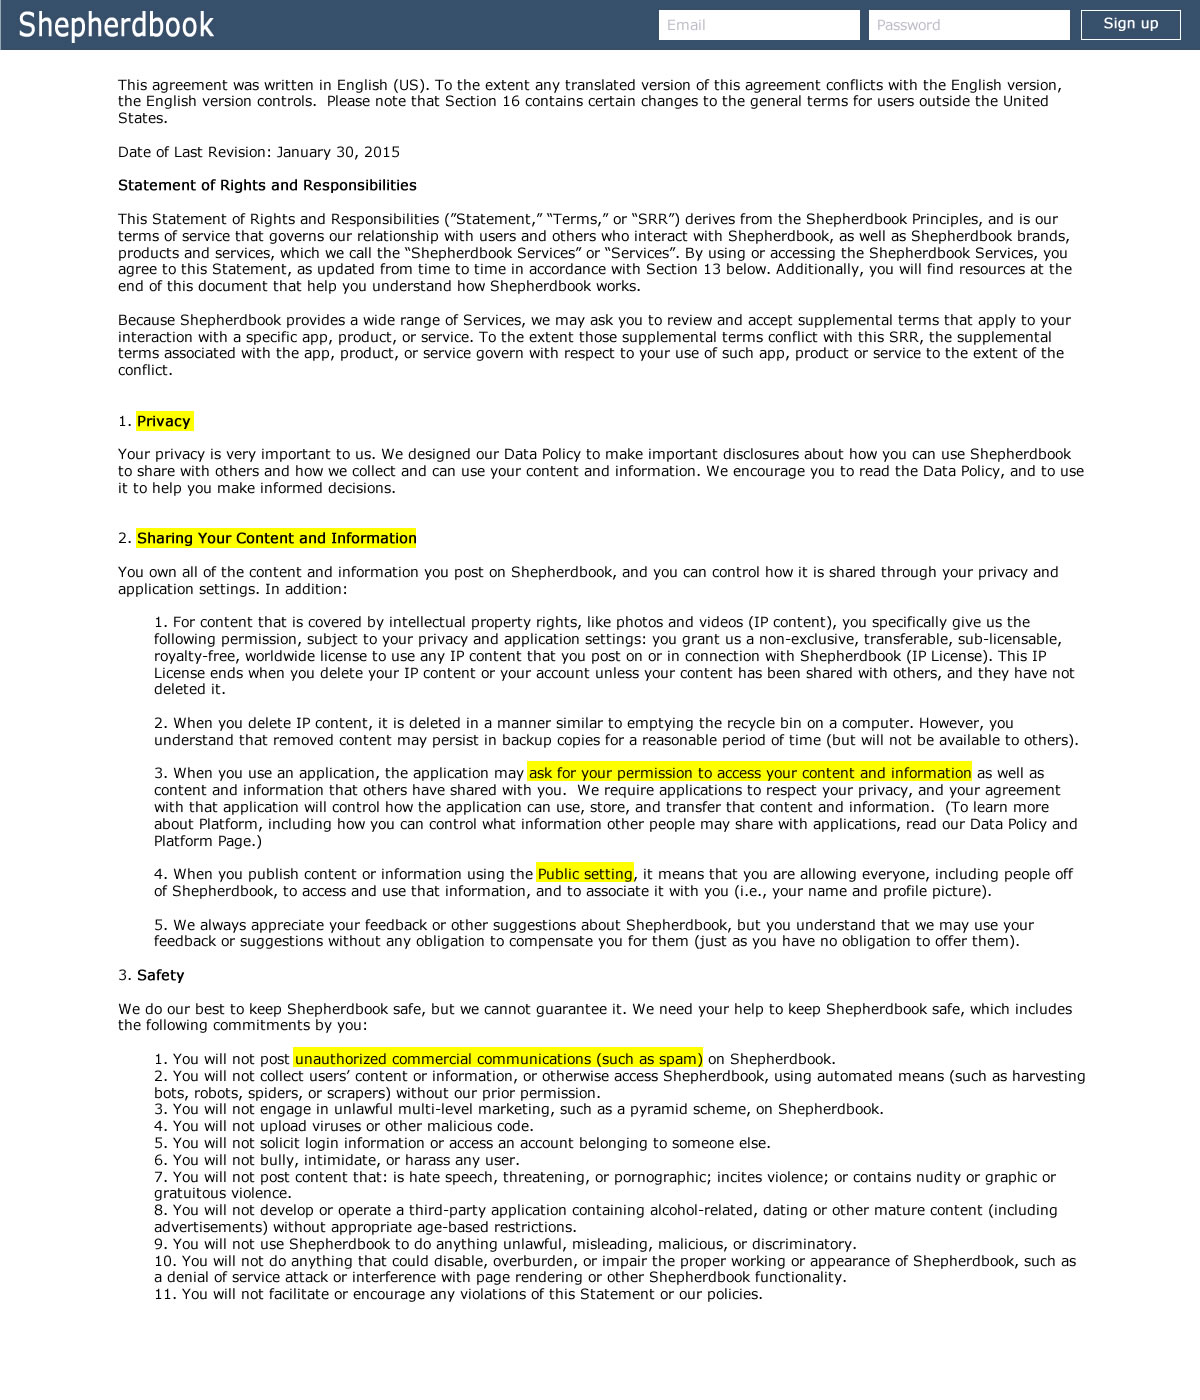
\includegraphics[width=1\columnwidth]{1_HighghtedTerms}
\caption{The highlighted words are considered as highly significant.}
\end{figure}

\paragraph{Mock-up 2}
In this mock-up, the community comments on the terms and agreements are 
presented. Those comments are shown to the user when he hovers or clicks on a 
highlighted item.

\begin{figure}[H]
\centering
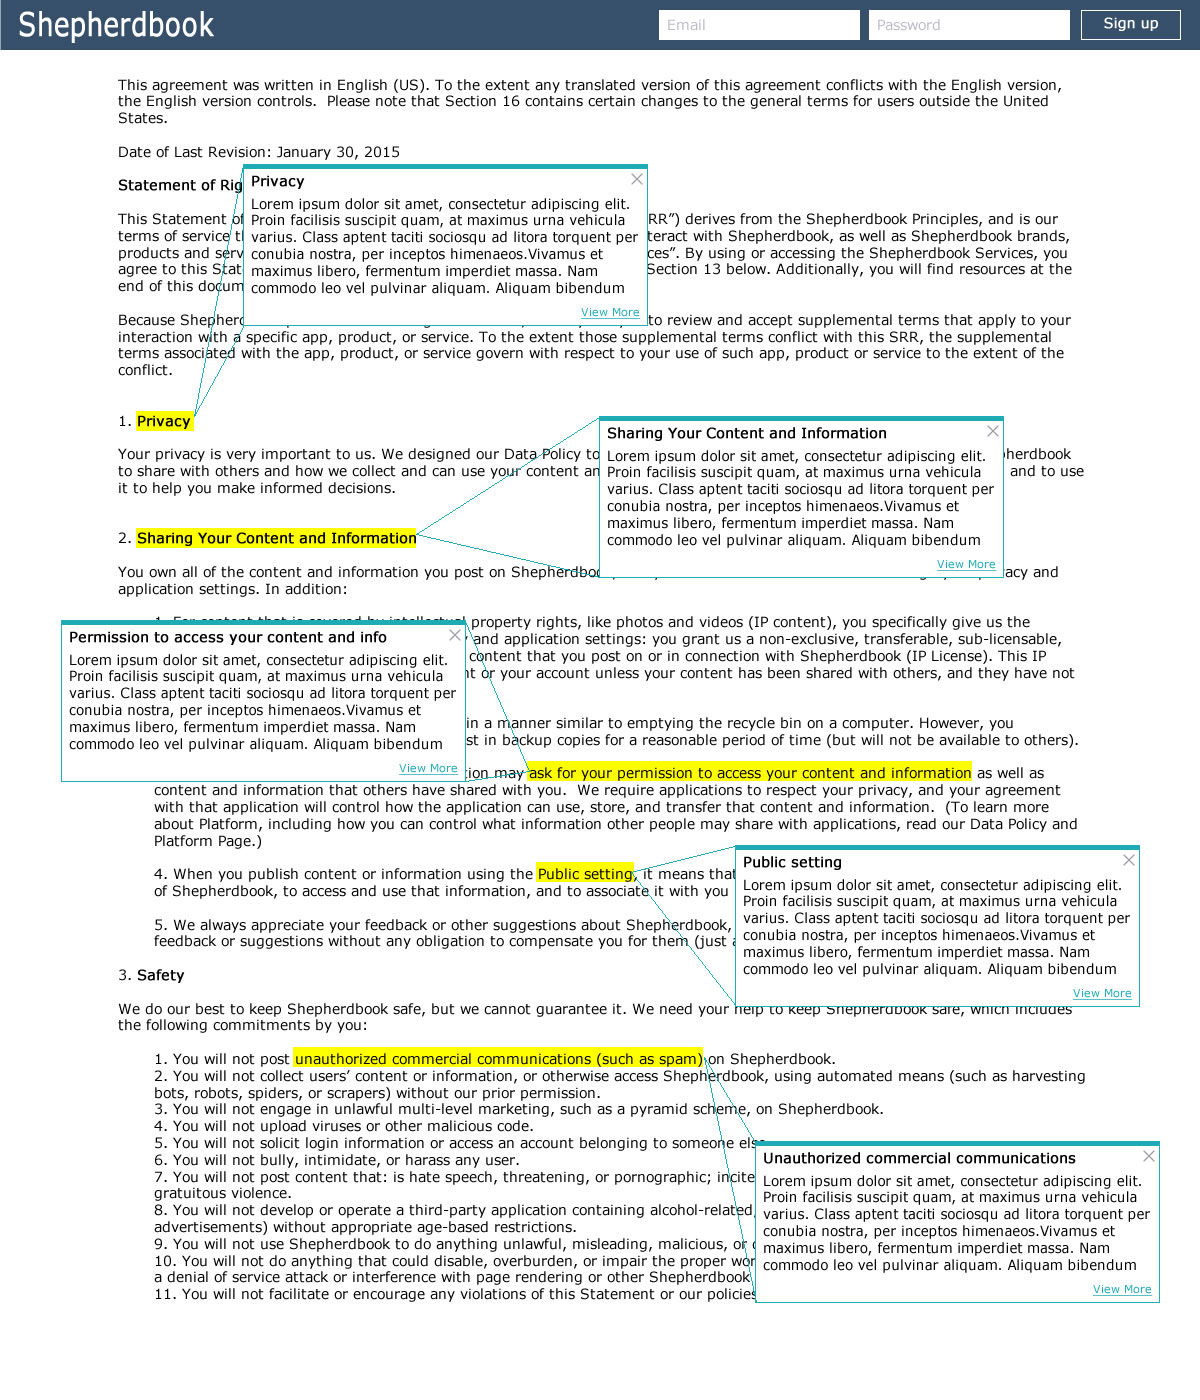
\includegraphics[width=1\columnwidth]{2_HighghtedTerms_Hover}
\caption{The community is responsible for the explanation of the highlighted 
text.}
\end{figure}



	\subsubsection{Prototype test planing}
\label{s_6}

For the prototype testing, we chose to ask five different people. This group of 
potential users is between 20 and 25 year-old university students, mixed female 
and male and derive from a diverse educational background. 
For our testing, we invited the selected group to the university study room, 
where the prototype test took place. We firstly introduced the users with our 
concept and presented the idea. As a second step we asked them to traverse 
through the prototypes and speak their thoughts aloud. Concurrently, we measured 
the time each one needed to understand how to use the system and understand the 
presented results of each action. After the test, we asked them individually to 
elaborate on their thoughts, what they particularly found interesting or what 
confused them and also encouraged them to propose alterations as they wished. 
Furthermore, the university study room seemed to be the perfect location for our 
test, since it was easily accessible for the students. In addition, the place 
was considered ideal and free of distractions. 
The meeting with the group was arranged at the end of the week, since the group 
of those people had a more flexible schedule.


	\subsection{Prototype feedback and evaluation presentation}

\paragraph{User evaluation 1}

The first user was quite technically savvy and when we presented the prototypes 
to him he had no trouble traversing through the different elements. He 
understood the concept well and he also quoted ``Ah! This is very helpful!''.

\paragraph{User evaluation 2}

The second user had quite similar educational background. Upon testing the 
product, he had no trouble understanding how to use it, but mentioned it was a 
bit overwhelming when all the comments popped up at once.

\paragraph{User evaluation 3}

The third user was from a completely different background than the previous two. 
It was noticed that it was more difficult to him to understand the concepts, but 
managed to finish the test in an affordable cost of time. Upon the completion of 
the test, he mentioned that even though the document was easier to understand, 
it still did not give him enough motive to start paying attention to the terms 
and agreements, because he consider it a boring and time consuming task anyway.

\paragraph{User evaluation 4}

This user found it quite confusing that all the comments popped up at the same 
time and proposed alterations, such as providing the comments one at a time or 
one after another, but make them not to occupy the full page.

\paragraph{User evaluation 5}

The last user traversed quite easily through the elements, even though he was 
not especially accustomed to such services. He commented that the idea was 
something that he himself would use in his everyday online activities and found 
it very helpful.

\subsection{Feedback outcome}

\paragraph{The good}

The majority of the users found our proposed add-on prototype very helpful and 
they would be willing to use it in the future. They pointed out that our idea 
was very interesting and significant, since ignoring the terms and agreements, 
nowadays, can prove to be very dangerous regarding the user's privacy. In 
addition, the existence of a wide open community behind this notion provides a 
sense of safety and assurance to the users (continuous updates, discussions, 
support, etc.). 

\paragraph{The bad}

As expected, the feedback contained also, some negative comments. Fortunately, 
the cons of our prototype were based on the appearance and the functionality of 
our add-on. The majority of the users felt that the comments on the highlighted 
sections might be significantly overwhelming and distracting, when in a large 
amount. 

\paragraph{The unexpected}

Surprisingly enough, one of the five users that we questioned stated that 
regardless the existence of our add-on and the functionality that it provides, 
he was not willing to use it. 
He specifically mentioned that reading and paying attention to the terms and 
agreements of each service or application is a loss of time. This is something 
very alarming, since it indicates that regardless the privacy preserving tools 
that exist in the wild, there are users that are not even interested in 
attempting using them.


	\subsubsection{Concept iterations}

The feedback phase proved to be very helpful regarding our prototype testing. In 
total, the users were significantly positive for our prototype proposal. They 
found the concept of our  idea very innovative, useful and mainly helpful. Thus, 
the feedback that we got was basically confident. However, since there are 
always opportunities for enhancements, the users gave some comments that would 
improve further the design and appearance of our prototype. The majority of the 
users pointed out that, sometimes, it was quite tough focusing on key points, 
when the amount of pop-ups was large. Taking this into consideration, we decided 
to reexamine the design of our prototype. Refinishing our mock-ups, we 
concentrated on presenting our add-on in a more simplistic, attractive and less 
overwhelming manner. We narrowed down our options and we concluded to show the 
comments only when the user mouse is over the highlighted words. With this 
approach, the pop-ups appear only ``upon request'' and the user is not 
overwhelmed with multiple windows. The rest of the design of our prototype 
remains the same as previously. 

	\subsection{Updated Concept Presentation}

\paragraph{Design Challenge} 

Refinement of terms and conditions in order to make them easier to read and more 
appealing to the users.

\paragraph{HMW Questions}

How might we make terms and conditions more legible for the casual users?

\paragraph{Description}

The basic idea is to create a service that will help identify the key parts of 
any online terms and agreements document. This service is based on the open 
source idea, both in development and maintenance. It uses a distributed database 
that contains keywords and key phrases, which is constantly updated, each time 
new laws, regulations, terms and agreements appear. This service will take the 
form of a web browser extension that upon request uses a web crawler will scan 
the document and match each recognised word or phrase retrieved from plain text 
with the ones in the database. Should any matches arise, they will be 
highlighted on the document. For the maintenance and update of this service, a 
user community is responsible. Every user of the service can also be a member of 
the community and can also provide comments on law sections or alterations and 
redefinitions on parts of the document. Every submitted comment by the community, 
will be displayed alongside the highlighted words and phrases in a pop up box 
when the user hovers or clicks each respective item.

\paragraph{Ideas Impact on the Challenge}

The main purpose of this challenge is to find ways to have more transparency on 
where our data is going on the internet. By developing this service, we enable 
users to have a better understanding of the rights they give to each service to 
handle their personal information. That way, before agreeing to use an online 
service, they will be able to know whether their data will stay private, used 
for external purposes or forwarded to third party services. To conclude, users 
can make their own decisions regarding their data, focusing on their privacy and 
not blindly agree to confusing terms because they purposely concealed their 
motives.

\subsubsection{Storyboard}

You can find our updated storyboard in the following link: 
\url{https://drive.google.com/open?id=1QnhbVuVnWkFZ8fuaYfQHeT_zflJqK_QtUoV57u9pI0k}.

\subsubsection{Mock-ups}

The mock-up below shows the updated version that takes into consideration the 
feedback of the users.
 
\begin{figure}[H]
\centering
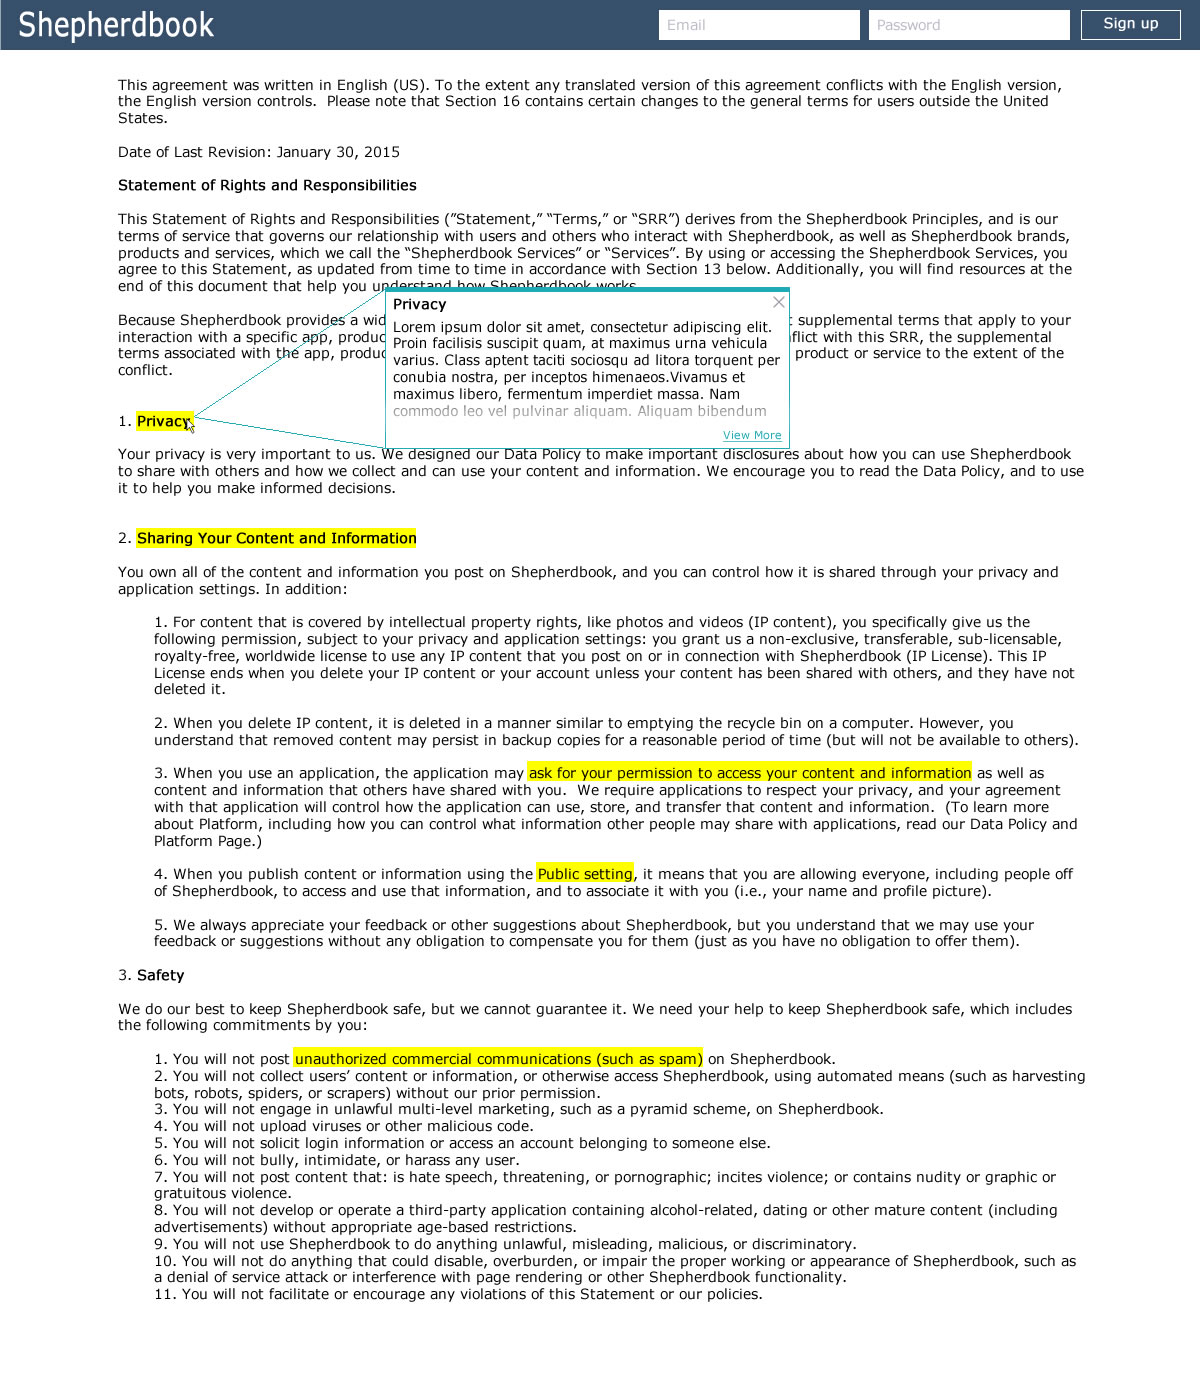
\includegraphics[width=1\columnwidth]{3_HighghtedTerms_Hover_Refined}
\caption{In the updated version, only one comment per highlighted text is shown.}
\end{figure}


	
	\section{Chapter 3: Implementation}
	\subsection{Action plan}

\subsubsection{Core skills}

Our team consist of two core parts.
The first one is the technical team, which contains the web developers 
responsible for the implementation of the web tool. The database will be 
operated by the back-end developers and the whole system will be maintained by 
the administrators and moderators. The latter are also responsible for the right 
functionality of the social part of the community (social media, forums, etc.).
Finally the UI designers will design all the needed web interfaces.

The second team is the economy and advertising group, which involves the economy 
experts, accountant. The economy experts are responsible for the evaluation of 
product costs and setting the goals in the direction of raising funds. On the 
other hand, the accountant is responsible for the distribution of money to each 
member of the team evaluating the economic worth of their work. Also, the 
accountant keeps track of the revenues and expenses in order to identify the 
needs of the project and the people that work for each development.

Finally, the manager is the key person behind the functionality and coordination 
of all the groups. The manager is the equal of a group leader, with exceptional 
people skills in order to motivate the team members and help the product rise. 
A good manager distributes the work equally, taking into consideration the 
capabilities of each individual in order to finally achieve the best possible 
result.

\subsubsection{Partnerships}

On every breakthrough idea partnerships are required in order for the idea to be 
supported. Those partnerships are divided into three categories.
First, support is needed from a marketing company. A good marketing agency may 
be able to help e-commerce businesses grow more quickly and alleviate stress for 
the entrepreneurs who own those businesses. It is common for online services and 
extensions to have Facebook pages, Twitter accounts, a YouTube or Google+ 
account, and maybe even an Instagram profile. This leads to an advertisement of 
the given service and resources to reach its full potential. By employing a 
marketing company that specializes in social media can save a significant amount 
of time and, possibly, generate better results.

Another partnership required is with a law firm. This is a partner, who can help 
deal with the difficulties in understanding the glossary used to form the terms 
and conditions document. An issue that is going to be resolved with this 
partnership is comprehension from the perspective of the user regarding the 
effects of accepting  terms and conditions of an online service.

Last but not least, our service needs a group of linguistic consultants. This 
group will help the service develop and grow to all possible users of each 
nationality. In addition, the linguists will help to redefine all the 
information that is going to be provided by the law firm in order to break it 
down to the level of users to understand what they are reading.

\subsubsection{Revenue and cost model strategy}

\paragraph{Funding}
First of all the project will be self funding from the team in order to create a 
basic demo implementation, that will be used for fund raising from crowd-funding 
sites. Crowd-funding platforms like Kickstarter and gofundme that 
gave life to many other projects like Pebble Time that raised over \$20.000.000 
from around 80.000 backers. That funding is needed for the operational costs 
like databases, site hosting, promotion and marketing. From that point forward 
the plug-in will be sustained from donations from users either if they are 
engaged with the community or not.

\paragraph{Costs}
The primary costs for the plug-in are the databases needed and the hosting for 
the community web servers. The code for the plug-in will be open source and 
public at github so anyone can contribute, removing the costs for the developers 
of any kind. As the project will be open source the different teams will not be 
paid directly by the project as they will contribute to the community as 
volunteers. Depending on the amount of funds raised, some specialists in 
advertising, promoting and legal acts will be hired.

\paragraph{Revenue}
As mentioned above the goal of the plug-in is to raise the awareness of the 
users and not to create a business. The revenue will be based on user donations, 
in order to cover the maintenance costs. For that reason the main goal of the 
community is to reach every user of the Internet by making them understand the 
impact that terms and agreements have on their privacy. Also, by allowing 
everyone to contribute to the expansion of the project can transform it to a 
more complete platform. This would offer a greater level of web transparency, 
engaging more users to the community and also sensitizing more to join our cause 
and help by donating.  


	\section{The pitch}

\subsection{The project overview}

Do you know who has access to your personal information? Are you aware of how 
much publicly exposed you are? Are you certain that your data is not being used 
for malicious purposes? There are many third party companies that can obtain 
your sensitive information and collect private data from many of the services 
you provided those data yourself. This can be further used to construct 
advertisements targeted for you or even purposefully create fake profiles using 
parts of your personal information. Are you aware that you are the one who gave 
all those companies permission to do so?

The aforementioned facts are stated in plain sight in every terms and agreements 
document of every online service, even though the words are disguised and 
presented in such ways that are difficult for an average user to extract the 
hidden meanings. Those documents are quite extended on purpose and that is a 
crucial reason users do not spend time on reading them and consequently missing 
those concealed statements. Due to this fact, we aim to improve the transparency 
between client and service provider by enabling users to understand what they 
agree to, by spending as little time as possible in studying the terms and 
agreements that are presented to them.

To achieve this goal, we propose a free browser extension tool, coming as an 
open source idea, that will be compatible with any modern browser (Google 
Chrome, Safari, Opera,Mozilla Firefox, Microsoft Edge) available for downloading 
and easy to use. The core idea is to provide a clear view of the key parts of 
terms and conditions documents that need the attention of the user using a 
simple and straightforward interface. By keeping it simple we facilitate the 
iteration through the document, only focusing on the vital points that most 
probably also contain disguised messages, such as user privacy, public exposure 
and sharing between companies.

On the front end, users will be presented with the exact terms and agreements 
page of each service, enhanced by our tool by highlighting keywords or key 
phrases, providing additional pop up comments for each highlighted section 
containing further explanation or alternative interpretation of each one. On the 
back end there will be a distributed database containing those words and phrases 
in order to be matched with the ones in the document after being identified from 
a plain-text crawler.

The plug-in code will be publicly available in full on a repository such as 
github in order for any developer to contribute to its refinement. In addition, 
any user can also contribute to the project by becoming a member of an open 
community established to update and maintain the database with further keywords 
and comments. The idea behind the community is to provide a user centric 
environment and safer overall feeling, in order to obtain and ensure the user 
trust in using our service. Concluding, our proposition is an ongoing never 
ending process that commits to improve and update along with every online 
service. 

\subsection{Pitch targets and objective}

Our plug-in extension tool is going to be pitched to two specific groups. The 
first group that is crucial to  pitch to are the users  

In the first category the target is to engage users to download and install the 
plug-in to their browser. In order to achieve that, our service needs to be 
presented in a certain way, which is going to alert the users about the 
significance of terms and agreements and the impact they have to their privacy. 
Another objective for pitching to the users is to make them immerse in the 
community. This step is important because the service is depending on the help 
of each user for improving the quality of the provided feedback given on terms 
and conditions.

The aspect of funding is another important factor which is going to be crucial 
for the development part of our service. Nowadays, various ways of funding exist 
for developing creative ideas. Our service is targeting a funding from 
KickStarter which can be used to raise the necessary amount of money for the 
starting operational costs. Furthermore, every user can contribute to the 
financial viability of the project by donations. 

\subsection{Elevator pitch}

``Hey! I have a brand new mobile phone. I’ll give it to you for free, do you 
want it? I bet you said yes without a second thought. What if I told you that 
without you noticing, it collects all your personal information? Do you still 
want it? No. Then why do you not pay attention to terms and conditions of use? I 
know it's boring. I can help you! Download and use my plug-in on your browser 
and let it automatically highlight the keywords on those tedious documents. You 
still don't trust me? Then trust the community that contributes to its accuracy 
and improvement with helpful comments. Is it clearer now? You can help others, 
too. Become a member, spread the word.''

%	\section{Brainstorm on potential solutions for your challenge, considering your 
synthesis output. No judgement here! Come up with at least 2 different solutions 
and provide a short summary of each.}
\label{s_1}

\paragraph{Solution 1: Refinement of terms and conditions in order to make them 
easier to read and more appealing to the users.} 
How to: Provide an add-on service that, by using a database containing keywords 
that are most commonly used in such documents, highlights those words in the 
terms and conditions document that each online service provides. In addition, as 
a further step, a user community will be established with the goal to refine 
such documents, and present them in parallel with the original document. The 
aforementioned refinement will provide the same document written in simpler 
words, to help users with little to no experience with law terms understand 
better the conditions they are asked to agree with.

\paragraph{Solution 2: Inform users about the risks of sharing sensitive and 
private information on social media and on online services in general.} 
How to: Produce a public video, available for sharing, that shows in a direct 
way how much private information can be collected for a random individual, just 
by peeking at his social media profiles. In this video, the lead actor will be a 
``mind reader'' who will offer to read a random passers by mind. At the same 
time a hidden assistant, after hearing the name of the ``victim'' will search to 
find every possible information he can and provide them by hidden earpiece to 
the ``mind reader'', who subsequently will present them as findings from reading 
the ``victim's'' mind. After the session is over, the hidden assistant will be 
revealed to make the ``victim'' realise that he was exposed through the stuff he 
willingly posted online.

\paragraph{Solution 3: Transparency on the user's information that can be 
extracted and used for profiling and how much they cost.} 
How to: Provide an add-on service, that every time you press/run it, it will gain 
all information it can extract from you and represent them in a table. This 
information will include your IP address, location, operation system, your 
personal computer's technical characteristics, the browser you use, search 
history, the online services you are currently logged in etc. In addition, this 
service will communicate with another, already existing service, that can 
compute the cost of an individual's personal information, and provide this as 
well.


%	\section{Cluster them into themes that you will define.}
\label{section_2}
Based on the findings, five different categories emerged. Those categories are:
\begin{enumerate}
\item
Privacy and anonymization tools
\item
Routing and storage
\item
Law enforcement and regulations
\item
Economy and advertising
\item
User trust
\end{enumerate}

%	\section{Turn your findings into ``insight statements''. Include a few insight 
statements under each theme.} 
\label{section_3}

\vspace{0.4cm}
\paragraph{Theme:} Privacy and anonymization tools.
\paragraph{Insights:}
\begin{enumerate}
\item
Users regardless of age or education level tend to care about their privacy on 
the internet.
\item
The majority of users believe that there isn't any stringency on user's internet 
data privacy.
\item
Even though users are willing to use anonymization tools for their protection on 
the internet, they seem reluctant to pay for such a service.
\end{enumerate}

%%
\vspace{0.1cm}
\paragraph{Theme:} Routing and Storage. 
\paragraph{Insights:}
\begin{enumerate}
\item
Most of the users seem to be concerned about their traffic routing and data and 
the specific storage locations.
\item
Users want to be more informed about the identity of third party companies 
interceding their communications.
\end{enumerate}

%%
\vspace{0.1cm}
\paragraph{Theme:} Law Enforcements and Regulations.
\paragraph{Insights:}
\begin{enumerate}
\item
Users tend to not pay attention to the ISPs terms and agreements regardless of 
the time they have spent on the internet. 
\item
More than half of users, care a lot about the sharing of their information to 
the law enforcement agencies and government.
\item
Users are not fully informed about the implication of laws of each country on 
their data.
\end{enumerate}

%%
\vspace{0.1cm}
\paragraph{Theme:} Economy and Advertising. 
\paragraph{Insights:}
\begin{enumerate}
\item
Users are fully aware of the existence of targeted advertising on the internet.
\item
Users are aware about profiling mechanisms on targeted advertising, and they are 
concerned about being the product of the internet advertising companies. 
\end{enumerate}

%%
\newpage
\paragraph{Theme:} User Trust. 
\paragraph{Insights:}
\begin{enumerate}
\item
Most of the users tend to not trust the ISPs with handling their personal 
information.
\item
A very high percentage of the users do not trust the social media to keep their 
information private.
\end{enumerate}



%	\section{Revisit your main challenge and refine it and its sub-questions, based 
on your insight statements.}
\label{section_4}

\paragraph{Insight: } 
Users tend to not pay attention to the ISPs terms and agreements regardless of 
the time they have spent on the internet. \\
\\\emph{How might we } 
refine terms and agreements more appealing to users and engage them more to pay 
attention to what they have agreed with?

\paragraph{Insight: }
Users are concerned about their profiling on targeting advertisement. \\
\\\emph{How might we }
restrict profiling to provide targeted advertising only on the services that 
will benefit us, regarding user budget and targeted recommendations (e.g. 
e-shops, airline tickets)?\\
\\\emph{How might we }
have more transparency on the exact information that are extracted to build the 
user profiles and their cost?

\paragraph{Insight: }
A very high percentage of the users do not trust the social media to keep their 
information private.\\
\\\emph{How might we }
inform users better about the risks of sharing sensitive information online?

\paragraph{Insight: }
Even though users are willing to use anonymization tools for their protection on 
the internet, they seem reluctant to pay for such a service.\\
\\\emph{How might we }
develop a reliable service that users can trust for security and privacy?

\paragraph{Insight: }
Users are not fully informed about the implication of laws of each country on 
their data.\\
\\\emph{How might we }
inform users about the existing laws of each country which apply to their online 
data and traffic.


%	\section{Present your concept in any other format, such as user experience 
diagram, mock-ups, flow charts, etc..}
\label{s_5}

\paragraph{Mock-up 1}
This mock-up represents the highlighted version of terms and agreement that the 
proposed plug-in will provide.

\begin{figure}[H]
\centering
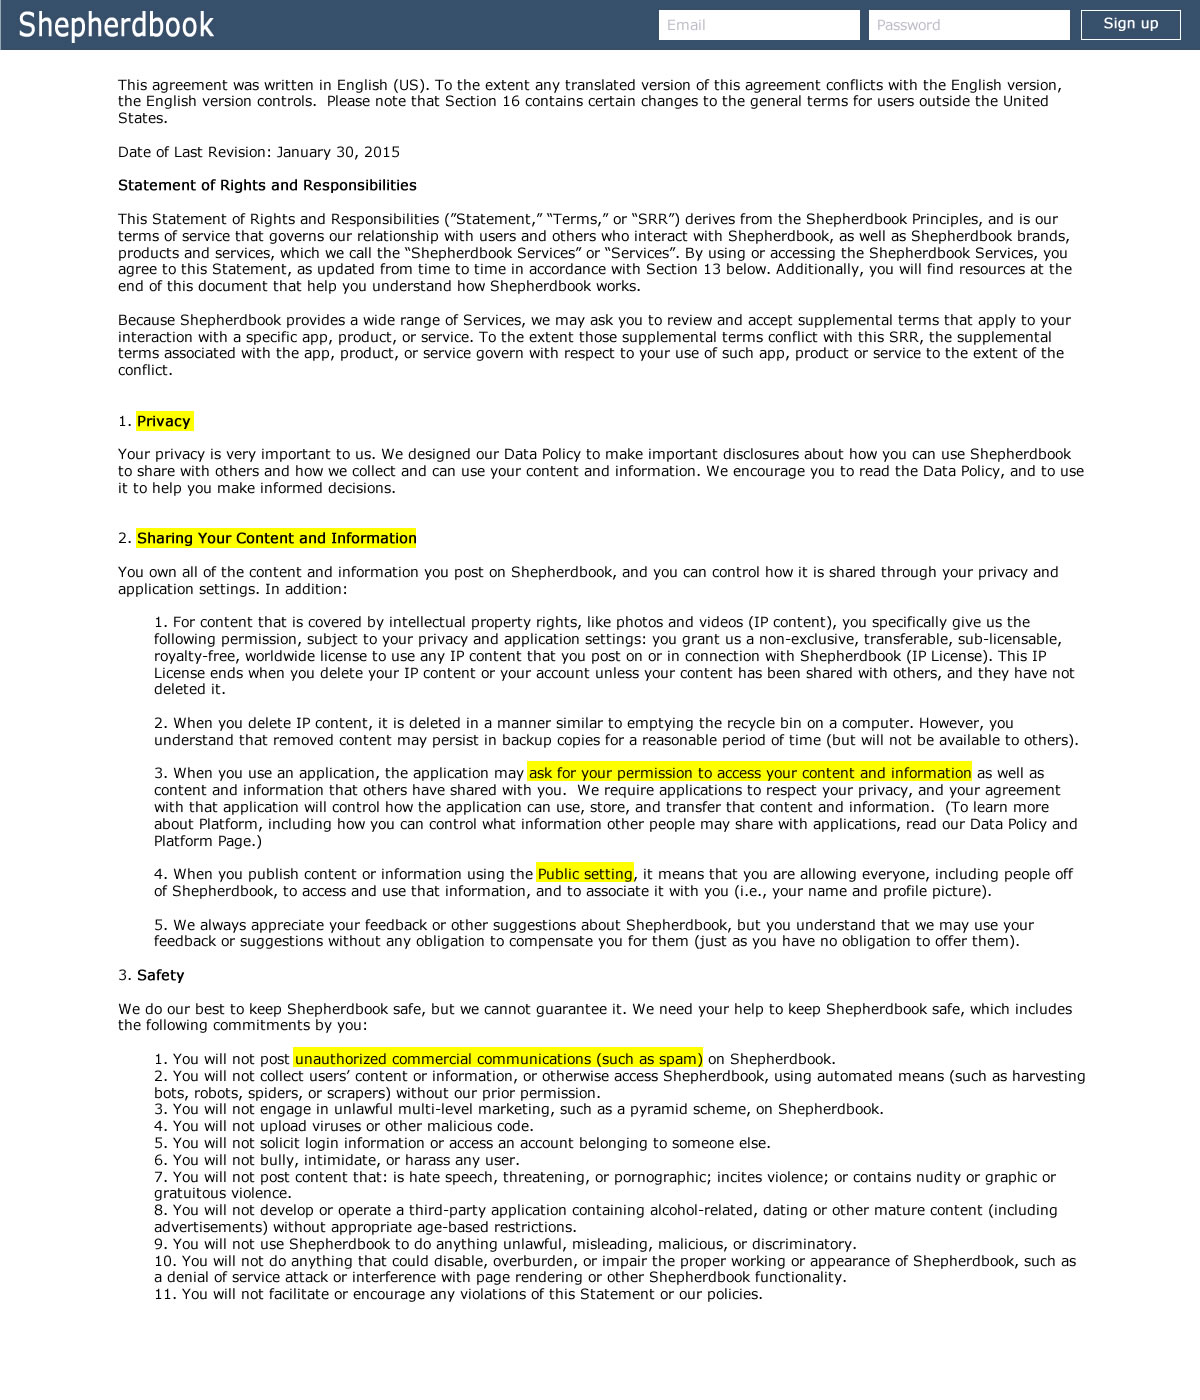
\includegraphics[width=1\columnwidth]{1_HighghtedTerms}
\caption{The highlighted words are considered as highly significant.}
\end{figure}

\paragraph{Mock-up 2}
In this mock-up, the community comments on the terms and agreements are 
presented. Those comments are shown to the user when he hovers or clicks on a 
highlighted item.

\begin{figure}[H]
\centering
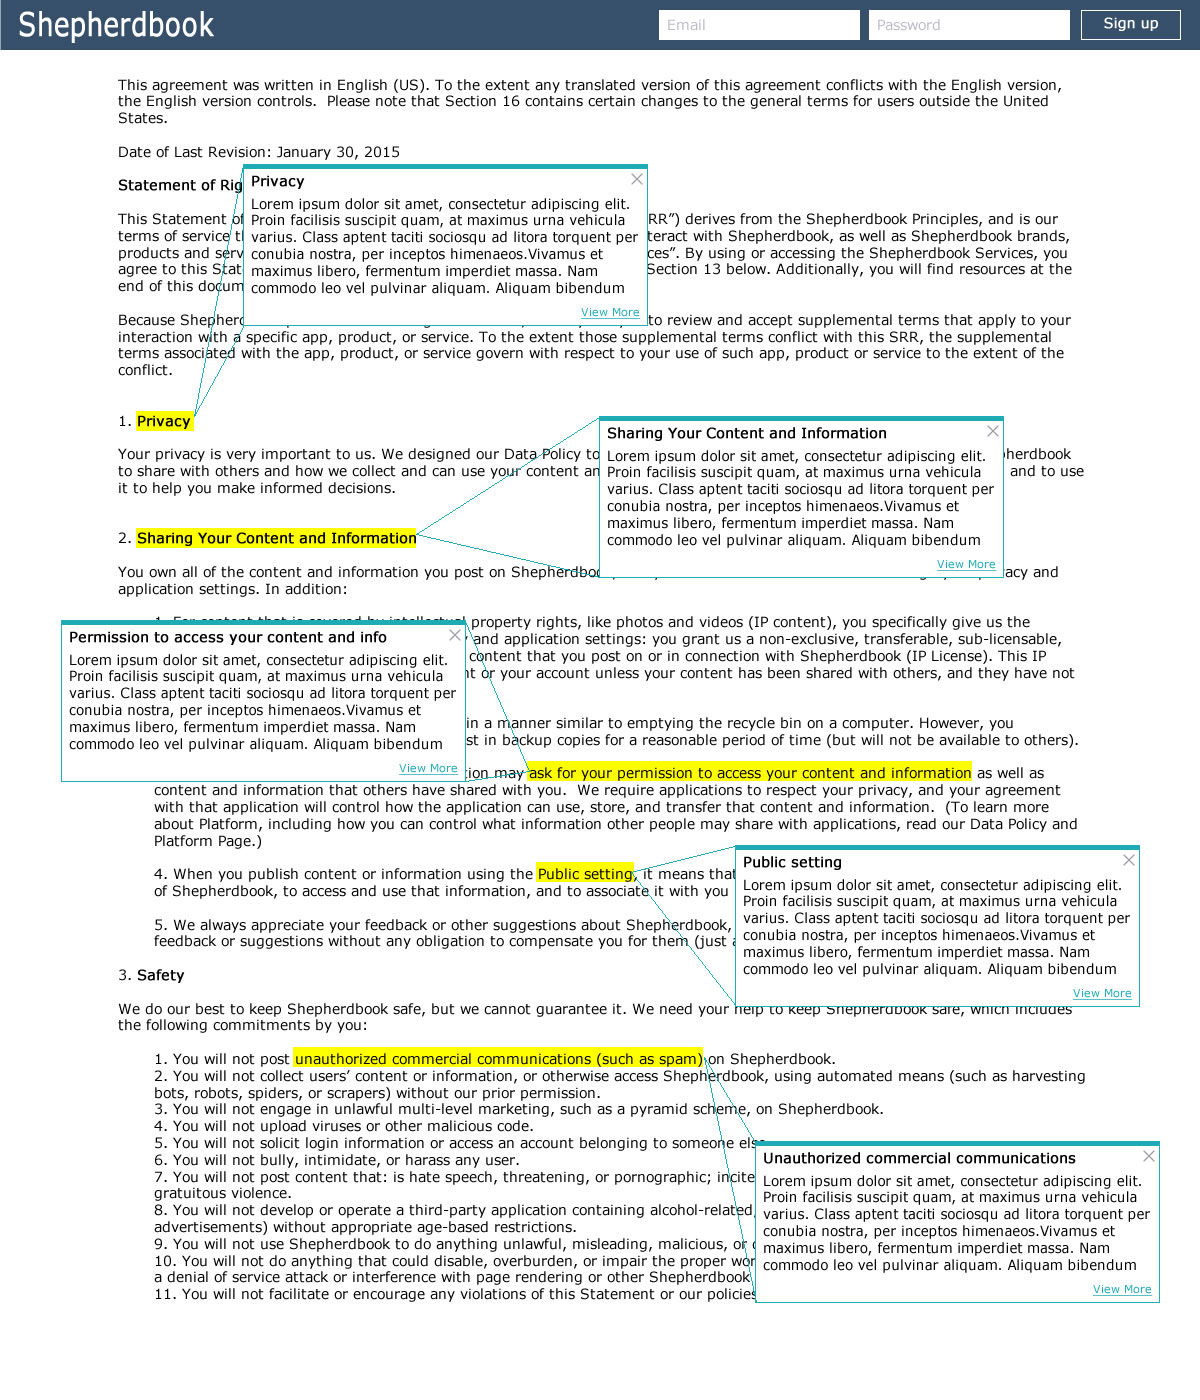
\includegraphics[width=1\columnwidth]{2_HighghtedTerms_Hover}
\caption{The community is responsible for the explanation of the highlighted 
text.}
\end{figure}



%	\section{Plan your prototype test: Who you will prototype with, how and when?}
\label{s_6}

For the prototype testing, we chose to ask five different people. This group of 
potential users is between 20 and 25 year-old university students, mixed female 
and male and derive from a diverse educational background. 
For our testing, we invited the selected group to the university study room, 
where the prototype test took place. We firstly introduced the users with our 
concept and presented the idea. As a second step we asked them to traverse 
through the prototypes and speak their thoughts aloud. Concurrently, we measured 
the time each one needed to understand how to use the system and understand the 
presented results of each action. After the test, we asked them individually to 
elaborate on their thoughts, what they particularly found interesting or what 
confused them and also encouraged them to propose alterations as they wished. 
Furthermore, the university study room seemed to be the perfect location for our 
test, since it was easily accessible for the students. In addition, the place 
was considered ideal and free of distractions. 
The meeting with the group was arranged at the end of the week, since the group 
of those people had a more flexible schedule.


%	\section{Present your prototype feedback and its evaluation. Present the GOOD, 
the BAD and the UNEXPECTED feedback you received.}
\label{s_7}

\subsection{User evaluations}

\paragraph{User evaluation 1: }
The first user was quite technically savvy and when we presented the prototypes 
to him he had no trouble traversing through the different elements. He 
understood the concept well and he also quoted ``Ah! This is very helpful!''.
\paragraph{User evaluation 2: }
The second user had quite similar educational background. Upon testing the 
product, he had no trouble understanding how to use it, but mentioned it was a 
bit overwhelming when all the comments popped up at once.
\paragraph{User evaluation 3: }
The third user was from a completely different background than the previous two. 
It was noticed that it was more difficult to him to understand the concepts, but 
managed to finish the test in an affordable cost of time. Upon the completion of 
the test, he mentioned that even though the document was easier to understand, 
it still did not give him enough motive to start paying attention to the terms 
and agreements, because he consider it a boring and time consuming task anyway.
\paragraph{User evaluation 4: }
This user found it quite confusing that all the comments popped up at the same 
time and proposed alterations, such as providing the comments one at a time or 
one after another, but make them not to occupy the full page.
\paragraph{User evaluation 5: }
The last user traversed quite easily through the elements, even though he was 
not especially accustomed to such services. He commented that the idea was 
something that he himself would use in his everyday online activities and found 
it very helpful.

\subsection{Feedback outcome}

\paragraph{The good: }
The majority of the users found our proposed add-on prototype very helpful and 
they would be willing to use it in the future. They pointed out that our idea 
was very interesting and significant, since ignoring the terms and agreements, 
nowadays, can prove to be very dangerous regarding the user's privacy. In 
addition, the existence of a wide open community behind this notion provides a 
sense of safety and assurance to the users (continuous updates, discussions, 
support, etc.). 
\paragraph{The bad: }
As expected, the feedback contained also, some negative comments. Fortunately, 
the cons of our prototype were based on the appearance and the functionality of 
our add-on. The majority of the users felt that the comments on the highlighted 
sections might be significantly overwhelming and distracting, when in a large 
amount. 
\paragraph{The unexpected: }
Surprisingly enough, one of the five users that we questioned stated that 
regardless the existence of our add-on and the functionality that it provides, 
he was not willing to use it. 
He specifically mentioned that reading and paying attention to the terms and 
agreements of each service or application is a loss of time. This is something 
very alarming, since it indicates that regardless the privacy preserving tools 
that exist in the wild, there are users that are not even interested in 
attempting using them.


%	\section{Present the iterations you made/will make to your concept.}
\label{s_8}

The feedback phase proved to be very helpful regarding our prototype testing. In 
total, the users were significantly positive for our prototype proposal. They 
found the concept of our  idea very innovative, useful and mainly helpful. Thus, 
the feedback that we got was basically confident. However, since there are 
always opportunities for enhancements, the users gave some comments that would 
improve further the design and appearance of our prototype. The majority of the 
users pointed out that, sometimes, it was quite tough focusing on key points, 
when the amount of pop-ups was large. Taking this into consideration, we decided 
to reexamine the design of our prototype. Refinishing our mock-ups, we 
concentrated on presenting our add-on in a more simplistic, attractive and less 
overwhelming manner. We narrowed down our options and we concluded to show the 
comments only when the user mouse is over the highlighted words. With this 
approach, the pop-ups appear only ``upon request'' and the user is not 
overwhelmed with multiple windows. The rest of the design of our prototype 
remains the same as previously. 

%	\section{Present your updated concept.}
\label{s_9}

\subsection{What is your design challenge and the respective HMW (how might we) 
question?}
\paragraph{Design Challenge: } 
Refinement of terms and conditions in order to make them easier to read and more 
appealing to the users.
\paragraph{HMW Questions: }
How might we make terms and conditions more legible for the casual users?

\subsection{Describe the idea and the impact it will have on the Challenge you 
have chosen (500 words or less).}

The basic idea is to create a service that will help identify the key parts of 
any online terms and agreements document. This service is based on the open 
source idea, both in development and maintenance. It uses a distributed database 
that contains keywords and key phrases, which is constantly updated, each time 
new laws, regulations, terms and agreements appear. This service will take the 
form of a web browser extension that upon request uses a web crawler will scan 
the document and match each recognised word or phrase retrieved from plain text 
with the ones in the database. Should any matches arise, they will be 
highlighted on the document. For the maintenance and update of this service, a 
user community is responsible. Every user of the service can also be a member of 
the community and can also provide comments on law sections or alterations and 
redefinitions on parts of the document. Every submitted comment by the community, 
will be displayed alongside the highlighted words and phrases in a pop up box 
when the user hovers or clicks each respective item.

The main purpose of this challenge is to find ways to have more transparency on 
where our data is going on the internet. By developing this service, we enable 
users to have a better understanding of the rights they give to each service to 
handle their personal information. That way, before agreeing to use an online 
service, they will be able to know whether their data will stay private, used 
for external purposes or forwarded to third party services. To conclude, users 
can make their own decisions regarding their data, focusing on their privacy and 
not blindly agree to confusing terms because they purposely concealed their 
motives.

\subsection{Present your Storyboard.}

You can find our updated storyboard in the following link: 
\url{https://drive.google.com/open?id=1QnhbVuVnWkFZ8fuaYfQHeT_zflJqK_QtUoV57u9pI0k}.

\subsection{Present your concept in any other format, such as user experience 
diagram, mock-ups, flow charts, etc..}

The mock-up below shows the updated version that takes into consideration the 
feedback of the users.
 
\begin{figure}[H]
\centering
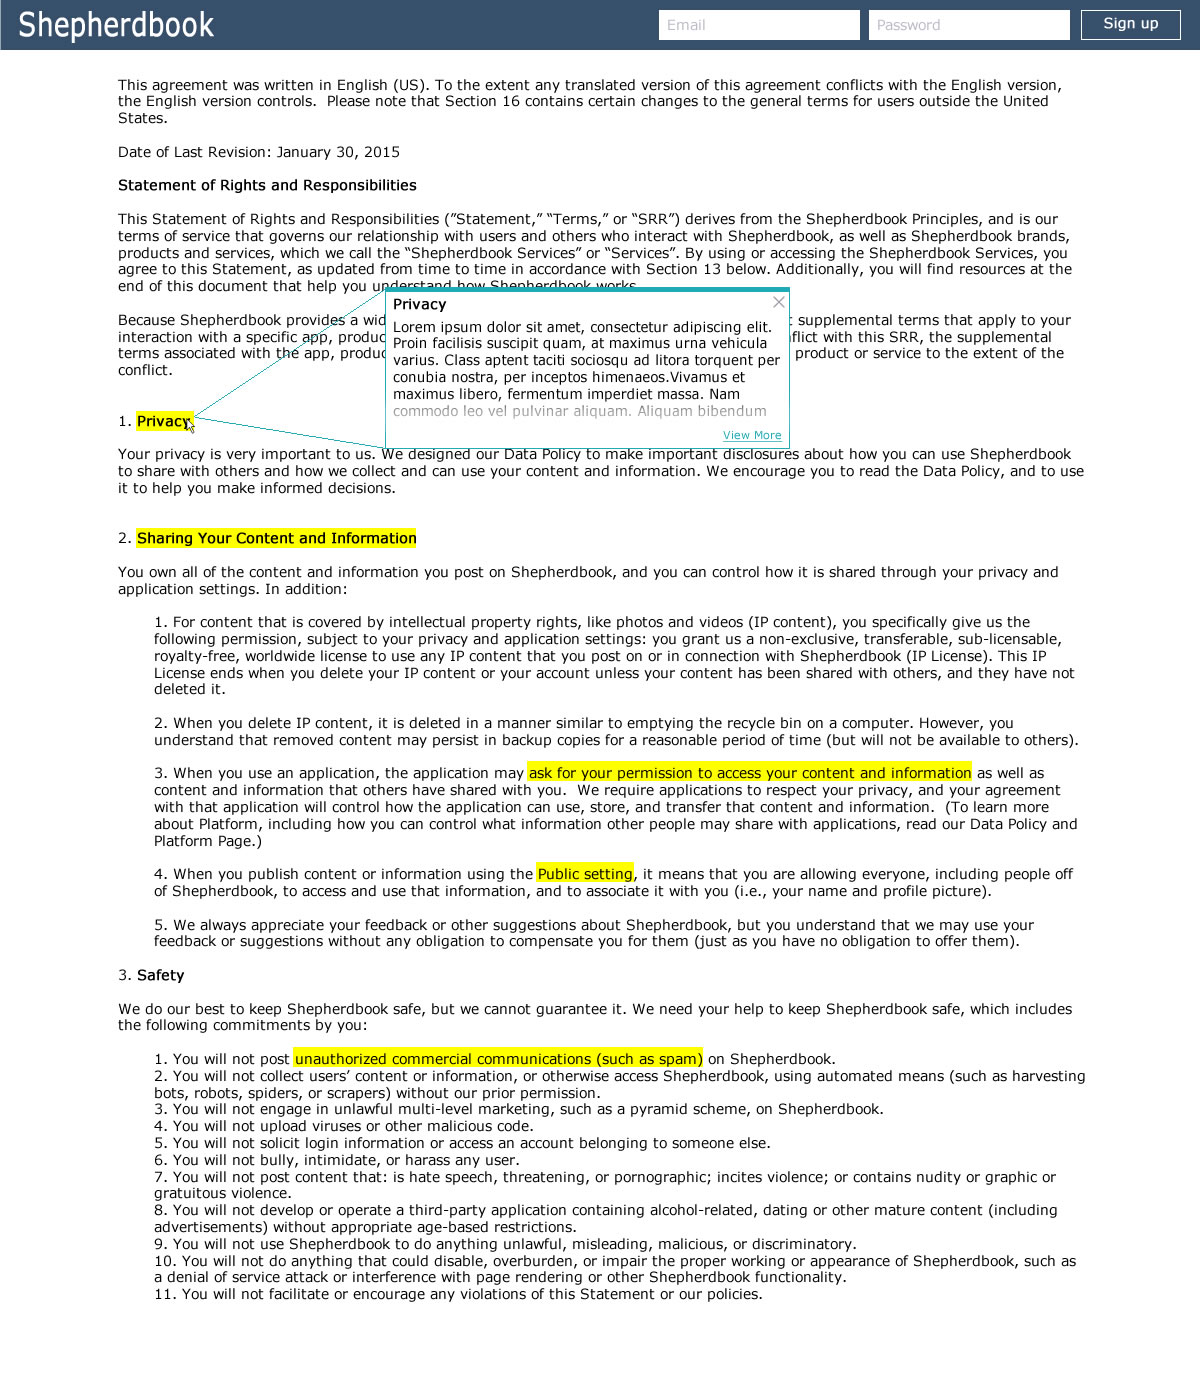
\includegraphics[width=1\columnwidth]{3_HighghtedTerms_Hover_Refined}
\caption{In the updated version, only one comment per highlighted text is shown.}
\end{figure}


	\section*{Acknowledgements}

We would like to thank Professor Xenofontas Dimitropoulos that accepted to be 
interviewed by our team in order to provide valuable feedback and information 
for this project. 
In addition, we would like to thank everyone that contributed to our project 
offering the time to answer our questionnaire.
Finally, we would like to show our gratitude to our mentors, Lefteris and 
Petroula, for their guidance. 



\end{document}
